% !TeX encoding = UTF-8
% !TeX spellcheck = en_US
% !TeX program = lualatex
\documentclass[xcolor={svgnames},10pt,
%notes,
handout
]{beamer}
\useoutertheme{metropolis}
\useinnertheme[sectionpage=progressbar,subsectionpage=progressbar]{metropolis}
\usefonttheme{metropolis}
%\usecolortheme{seahorse} 
%\usecolortheme{dolphin} 
\usecolortheme{metropolis}
\setbeamertemplate{note page}[plain]
%\usepackage{lmodern}
%\usepackage[utf8]{inputenc}
%\usepackage[T1]{fontenc}
%\usepackage{fontspec}
\graphicspath{{graphics/}}
\usepackage{csquotes}
\usepackage{textcomp}
\usepackage{listings}

\lstset{%
	language=R,                     % the language of the code
	basicstyle=\small, % the size of the fonts that are used for the code
%	numbers=left,                   % where to put the line-numbers
%	numberstyle=\tiny\color{DarkBlue},  % the style that is used for the line-numbers
	stepnumber=1,                   % the step between two line-numbers. If it is 1, each line	% will be numbered
	numbersep=5pt,                  % how far the line-numbers are from the code
%	backgroundcolor=\color{white},  % choose the background color. You must add \usepackage{color}
	showspaces=false,               % show spaces adding particular underscores
	showstringspaces=false,         % underline spaces within strings
	showtabs=false,                 % show tabs within strings adding particular underscores
	frame=single,                   % adds a frame around the code
	rulecolor=\color{black},        % if not set, the frame-color may be changed on line-breaks within not-black text(e.g. commens (green here))
	tabsize=2,                      % sets default tabsize to 2 spaces
	captionpos=b,                   % sets the caption-position to bottom
	breaklines=true,                % sets automatic line breaking
	breakatwhitespace=false,        % sets if automatic breaks should only happen at whitespace
	upquote=true,
	keywordstyle=\ttfamily,      % keyword style
	commentstyle=\color{DarkGreen},   % comment style
%	identifierstyle=\ttfamily,
%	stringstyle=\color{DarkGreen},      % string literal style
	keywords={},
	columns=fullflexible,
	literate=*{-}{-}1
} 


\begin{document}

\title[Introduction to R]{Introduction to R}
\author{Dr.\ Willi Mutschler }
\date{~}
\institute{}
\maketitle

\section{Introduction}

\begin{frame}
\frametitle{Aims and prerequisites}
\begin{itemize}
\item Objective: Learn how to use R for econometrics and statistics
\item Prerequisites:
\begin{enumerate}
\item Basics in probability theory and statistical inference
\item Multiple linear regression
\end{enumerate}
\end{itemize}
\end{frame}


\begin{frame}
\frametitle{References}
All materials and their source-codes are freely available online:
\begin{footnotesize}
\begin{description}
\item \url{https://github.com/wmutschl/IntroR/tree/IW}
\end{description}
\end{footnotesize}
Course is based on
\begin{itemize}
\item Introductory courses held at the Econ Department at University of Münster
\item Introductory courses on datacamp.com
\item Andreas Behr and Ulrich P\"{o}tter (2011): \emph{Einf\"{u}hrung in die Statistik mit R}
\item Muenchen, Hilbe (2012): \emph{R for Stata Users}
\end{itemize}
\end{frame}

\begin{frame}
\frametitle{Topics}
\begin{enumerate}
\item What is R?
\item R-Studio Basics
\item Managing workspace and packages
\item Get help and understand the documentation
\item Programming language basics
\item Controlling functions
\item Data structures and acquisition
\item Selection and transformations of variables and observations
\item Treatment of missing values
\item Data visualization (basic and using gramar)
\item Regression analysis
\item Programming
\end{enumerate}
\end{frame}


\section{What is R?}

\begin{frame}[standout]
\frametitle{What is R?}
\begin{itemize}
	\item[] \enquote{The most powerful statistical computing language on the planet...}
\end{itemize}
\end{frame}

\begin{frame}
\frametitle{What is R?}
It all depends on the use and user, BUT: R is
\begin{itemize}
\item an intuitive interface to the most advanced statistical methods available today
\item built specifically for data analysis and visualization
\item one of the most popular languages for data science
\item preferred by statisticians and academic researchers
\item language of choice for cutting edge statistics
\item a vast collection of community-contributed packages
\end{itemize}

\end{frame}

\begin{frame}
\frametitle{What is R?}
\begin{itemize}
\item The language S (an object-oriented statistical computing language) is implemented as S-Plus (commercial) and R (OpenSource)
\item R is a
\begin{enumerate}
	\item language
	\item package
	\item environment
\end{enumerate}
for graphics and data analysis
\item R is FOSS (think about collaborations!) and easily extendable
\item Similar programming languages: Matlab, GAUSS, Julia
\end{itemize}
\end{frame}
\note{
The differences between S-Plus and R are minimal\\
}

\begin{frame}\frametitle{Comparison to STATA}
In general, five independent parts of a software
\begin{itemize}
\item Data input and management (language)
\item Statistics and graphics procedures (commands)
\item Output management systems
\item Macro language
\item Matrix language
\end{itemize}
$\hookrightarrow$In other softwares, e.g. Stata, these are standalone and developed separately

$\hookrightarrow$In R all five were planed to be unified from the beginning
\end{frame}
\note{Output management systems: Stata return codes, postestimation, Matrix language in Stata is Mata}

\begin{frame}\frametitle{Comparison to STATA}
\begin{itemize}
\item \texttt{Base R} plus recommended packages contains over 1600 functions similar to e.g. STATA
\item Tested via extensive validation programs
\begin{itemize}
\item[$\hookrightarrow$] R is accurate even though no company behind it, R responds very quickly to bugs etc.
\item[$\hookrightarrow$] Source code of R (\textit{scripts}) are similar to \textit{Do Files} in STATA
\end{itemize}
\item Note that new statistical methods are nowadays often first published in R, and only later included by PROGRAMMERS (not original scientists) into STATA
\end{itemize}
\note{This has pro and cons}
\end{frame}

\begin{frame}[fragile]
\frametitle{R Console}\small
The basic command window is called the \texttt{R Console}\\
Prompt: \texttt{>}\\
You can input commands and execute them (by pressing the \textsc{Return} key)
\begin{lstlisting}
1+1
1+1 # This is a comment: 1+1
(1+2)*3
(5/3)^4.5
5+2; 7+3; 2*5
pi
Pi
PI
2*((1+2)*(1-2)
\end{lstlisting}
This will: (1) evaluate it, (2) print the result, (3) count the lines with [n] and (4) delete the result
\end{frame}
\note{That a plus sign appears if we forget to close paranthesis.
	
Upper and lower cases, dot and comma: R differentiates between upper and lower cases, try:
pi, Pi und PI. Keep that in mind when calling functions and commands, and also when naming
variables. 

The decimal point is the dot.
}

\begin{frame}
\frametitle{Editors}
\begin{itemize}
	\item Long computations should not be done interactively in the command	window
	\item Use an editor to write a program and then execute it in R
	\item There is a built-in editor in R: \texttt{Datei -- Neues Skript}
	\item External editors:
	\begin{itemize}
		\item \textbf{R-Studio [RECOMMENDED!]}
		\item Tinn-R, Notepad++, Atom, Emacs, etc. are also possible
	\end{itemize}
\end{itemize}
\end{frame}

\begin{frame}
\frametitle{R-Studio}
\begin{itemize}
	\item Overview of four panels in R-Studio:
	\begin{enumerate}
		\item Script editor
		\item Environment|History|Connections,
		\item Console|Terminal
		\item Files|Plots|Packages|Help|Viewer
	\end{enumerate} 
	\item Important shortcuts (see also the Magic Wand)
	\begin{itemize}
		\item ~[CTRL+ENTER] for Run
		\item ~[CTRL+SHIFT+C] for commenting a section
		\item ~[CTRL+L] clears command windows
		\item ~[TAB] Function completion
		\item ~[ARROWS UP AND DOWN] in command window: scroll through history
		\item ~[F1] gets you help
	\end{itemize}
\end{itemize}
\end{frame}
\note{One can change this layout as one sees fit in the options interface

Actually R-Studio can also be run on a server easily such that one could call rstudio.mutschler.eu}


\begin{frame}[fragile]
\frametitle{Concatenation, Assignments, Strings}\footnotesize
Open a new Script in R-Studio and try out the following:
\begin{lstlisting}
c(1,4,7)
a <- c(1,4,7)
print(a)
a
A
b <- c(1,a,3)
(b <- c(1,a,3))
mean(b)
simpsons_kids <- c( #family name
"Bart",           #boy name
'Lisa',           #girl name
"Maggie"          #baby name
)
print(simpsons_kids)
c(2,"3") -> y
\end{lstlisting}
Execute a single line (or multiple lines by marking them) by pressing \textsc{CTRL-ENTER}\\
\end{frame}
\note{
Variables are case-sensitive, e.g. pi, Pi, PI

Assignments: evaluate expression and store result <- ("gets"), = works to but avoid it
you can enter command with semicolon or separate commands, but usually just new line

a + at the command line indicates that a command is not complete, either complete it or hit ESC, - if you did not complete commands, you get a +, mostly ), or hit ESC key or STRG/CMD+C

}

\begin{frame}[fragile]
\frametitle{Concatenation, Assignments, Strings}

\begin{itemize}
	\item \lstinline|c()| is the concatenation operator and probably the most used command in R
	\item \lstinline|<-| and \lstinline|->| assign values to variables, you could also use \lstinline|=| but it is not recommended
	\item if you did not complete commands, you get a \lstinline|+|. Most of the times close a \lstinline|)|, or hit ESC key or CTRL+C
	\item comments go from \lstinline|#| to the end of line, can be between functions or in the middle with line breaks
	\item there is no block comment features, simply use [CTRL-SHIFT-C] in R-Studio to (un)comment sections
	\item Use either double quotation marks (\lstinline|"some string"|) or single ones (\lstinline|'some other strings'|). Note that double quotes are preferred (and output is printed using double quotes)
\end{itemize}
\end{frame}
\note{Copy and pasting of R commands from these slides often does not work (especially quotation marks and minus signs), depends on pdf reader, better type commands on your own!
}

\begin{frame}[fragile]\frametitle{Parenthesis}
(Parenthesis)
\begin{itemize}
	\item control math order as usual in algebra, e.g.
	\begin{lstlisting}
	1+1*10
	(1+1)*10
	\end{lstlisting}
	\item print assignment values: 
	\begin{lstlisting}
	(x<-c(1,2,3,4,NA))
	\end{lstlisting}
	\item provide options to functions, e.g.
	\begin{lstlisting}
	mean(x, na.rm=FALSE)
	mean(x, na.rm=TRUE)
	\end{lstlisting}
\end{itemize}
\end{frame}

\begin{frame}[fragile]\frametitle{Parenthesis}
\{Curly Braces\}
\begin{itemize}
\item Can combine many commands into one
\item Executes all assignments but returns only value of last expression
\item Useful for writing own functions
\begin{lstlisting}
{x<-2; y<-1
z<-x+y; z2<- z^2
z
z2}
\end{lstlisting}
\end{itemize}
[Square Braces] and [[Double Square Braces]]
\begin{itemize}
\item Used for selecting/indexing elements within objects (we will get to that later)
\item Double squares are used in lists (one of the most general data structure)
\end{itemize}
\end{frame}
\section{Managing workspace}



\begin{frame}[fragile]
\frametitle{Managing workspace}
Listing Objects
\begin{itemize}
\item \lstinline|ls()| or \lstinline|objects()| lists the objects in your workspace
\item \lstinline|rm(list=ls())| clears workspace
\end{itemize}
Working Directory
\begin{itemize}
	\item Easiest: Use GUI, i.e. Session - Set Working Directory
	\item alternatively: \lstinline|getwd()| and \\\lstinline|setwd("c:/Users/wmutschl/Documents/RKurs")| (PC)\\ \lstinline|setwd("/Users/wmutschl/Documents/RKurs")| (Mac)\\ \lstinline|setwd("/home/wmutschl/Documents/RKurs")| (Linux)
	\item Note that the path name is structured by slashes (\lstinline|/|), not backslashes (\lstinline|\|)
\end{itemize}
\end{frame}
\note{Special R Files: Rproj that remebmers the open files an working directory, stores settings in a folder named .Rproj.user
	R looks for the folowing files: .Rprofile (like profile.do) commands are automatically executed at startup (not a good practice)
	.Rhistory history of all statements! click on history tab, or history()
	.Rdata (not good)

SAve as
save.image(file="file.RData")
save(mydata,mylist,mymatrix,file="mypractice.RData")
Save WOrkspace image --> creates .RData in the current wd, when you start it will load it automatically, (TOOLS OPTION GENERAL, what you want)


}

\begin{frame}[fragile]
\frametitle{Managing workspace}
Quitting
\begin{itemize}
	\item Quit R by the command \lstinline|q()|
	\item Quit RStudio by using the GUI or [CTRL+Q]
	\item In general, save your script files, but do \emph{not} save your workspace
	\item Note that in RStudio even unsaved script files are kept
\end{itemize}
\end{frame}


\section{Packages}

\begin{frame}
\frametitle{Packages}
\begin{itemize}
	\item One of the strengths of R is the large and growing collection of packages that can be downloaded from CRAN (or e.g. Github)
	\item Installation (only once!)
	\begin{itemize}
	\item Use R-Studio interface for Packages
	\item \lstinline|install.packages("packagename")|
	\end{itemize}
	\item Installed packages are activated by \lstinline|library("packagename")|
	\item Help about packages: \lstinline|library(help="packagename")|
\end{itemize}
\end{frame}
\note{
Actually, library does not need quotations, but who cares.
}

\begin{frame}[fragile]
\frametitle{Common problems}
\begin{itemize}
\item \lstinline|install.packages("ggplot")|
	\begin{itemize}
	\item[$\hookrightarrow$] either not available or wrong package name 
	\end{itemize}
\item \lstinline|install.packages(ggplot2)|
	\begin{itemize}
	\item[$\hookrightarrow$] forgot quotes
	\end{itemize}
\item \lstinline|library("prettyR")|
	\begin{itemize}
	\item[$\hookrightarrow$] forgot to install it
	\end{itemize}
\item \lstinline|library("dplyr")|
	\begin{itemize}
	\item[$\hookrightarrow$] masked or covered up, that's okay
	\end{itemize}
\item \lstinline|detach("package:dplyr")| is opposite of library, which might prevent conflicts in function names and save on memory
\end{itemize}
\end{frame}

\begin{frame}
\frametitle{Which packages to use?}
\begin{itemize}
\item The Comprehensive R Archive Network (CRAN): can be searched by name or via Task Views for key programs on \texttt{cran.r-project.org}
\item \texttt{crantastic.org}: rated software
\item \texttt{rdocumentation.org}: top packages
\item \texttt{r-bloggers.com}
\item Git[hu|la]b, ...
\end{itemize}
\end{frame}

\begin{frame}[standout]
Exercise 1
\end{frame}
\section{Help and documentation}

\begin{frame}[fragile]
\frametitle{Help and documentation}
\begin{itemize}
	\item To obtain details about a command, type\\ \lstinline|?command| or \lstinline|help(command)|
\begin{lstlisting}
?mean
help(mean)
help("for")
help("while")
?"while"
help(package = "prettyR")
methods(plot) #gives you overview of extra functions, e.g. 
help(plot.lm)
help.start()
\end{lstlisting}
\item R-Studio: select/click on a command and hit F1
\end{itemize}
\end{frame}
\note{Some commands belong to a certain package or base, and need to be asked for with quotation marks}

\section{Programming Language Basics}

\begin{frame}[fragile]
\frametitle{R objects}
\begin{itemize}
\item R is object oriented
\item An object can be anything: scalar, vector, matrix, string, table, factor, list, data frame, regression results, model, \ldots
\item object name should begin with letter, no numbers, no underscores, no special characters, case matters
\item The object type determines how some commands work (e.g. \lstinline|plot|, \lstinline|summary|)
\item Every object has a unique name
\end{itemize}
\end{frame}




\begin{frame}\frametitle{Variables}
All kinds of values can be stored in a variable (as we are object-oriented):
\begin{itemize}
\item numbers
\item letters
\item words
\item dates
\item logical TRUE/FALSE values
\item data structures
\item plots
\item other objects
\item ....
\end{itemize}
\end{frame}


\begin{frame}[fragile]\frametitle{Mode, Class, Dimension and Length of Vectors}
\begin{lstlisting}
x <- c(1, 2, 1, 2, 1, 2, 1, 2)
print(x); mode(x); class(x); length(x); dim(x)
x+x
2*x
x + 10
x + c(10, 100)
x <- as.matrix(x)
print(x); mode(x); class(x); length(x); dim(x)
\end{lstlisting}\pause
\footnotesize
\begin{itemize}
	\item \lstinline|mode|: a variable's type
	\item \lstinline|class|: vectors have a class of character or numeric (or many other things), dimension (\lstinline|dim|) of a vector is NULL
	\item \lstinline|length|: number of elements it contains (including (!) missings)
	\item Note: If one vector is shorter, its values are \textbf{recycled} until the lengths match
\end{itemize}
\end{frame}
\note{Advantage of recycling: saves you typing, Disadvantage: might lead to errors. Attention: a vector is NOT a 1D-vector! Use \lstinline|as.matrix| instead!
}

\begin{frame}\frametitle{Operators and functions}
Logical operators
\begin{description}
\item[\texttt{\&}] and
\item[\texttt{|}] or
\item[\texttt{!}] not
\item[\texttt{NA}] not available or no answer
\item[\texttt{==}] equal (do \emph{not} use \texttt{=})
\item[\texttt{>}, \texttt{>=}] greater than,
greater than or equal
\item[\texttt{<}, \texttt{<=}] less than, less
than or equal
\item[\texttt{!=}] not equal
\end{description}
\end{frame}


\begin{frame}[fragile]
\frametitle{Operators and functions}
Examples logical operators
\begin{lstlisting}
5 < 7
1+1 == 3
a <- c(-1,4,9)
a >= 2 & a < 8
b <- c(NA,1,2,3)
b > 0
is.na(b)
a[a>2]
a == 4
a = 4
\end{lstlisting}

\end{frame}

\begin{frame}[standout]
Exercise 2
\end{frame}


\begin{frame}\frametitle{Operators and functions}
Arithmetic operators and mathematical functions
\begin{description}
\item[\texttt{+}, \texttt{-}] plus, minus
\item[\texttt{*}, \texttt{/}] multiplication and division
\item[\texttt{\symbol{94}}] power (exponentiation)
\item[\texttt{Inf}, \texttt{-Inf}] infinity (plus or minus)
\item[\texttt{NaN}] not a number
\item[\texttt{abs}] absolute value
\item[\texttt{sqrt}] square root
\item[\texttt{exp,log}] exponential function and natural logarithm (\emph{not} \texttt{ln})
\item[\texttt{sin}] sinus (other trigonometric functions as well)
\item[\texttt{sum}] sum
\end{description}
\end{frame}


\begin{frame}[fragile]
\frametitle{Operators and functions}
Examples arithmetic operators and mathematical functions
\begin{lstlisting}
x <- c(-1,0,2,9,3)
abs(x)
sqrt(x)
1/x
-1/x
0/x
log(x)
x^c(2,3,2,3,2)
x^c(2,3)
log(x)<0
\end{lstlisting}
\end{frame}


\begin{frame}[standout]
Exercise 3
\end{frame}


\begin{frame}
\frametitle{Operators and functions}
Matrix functions
\begin{description}
\item[\texttt{matrix}] creates a matrix from a vector
\item[\texttt{dim}] dimensions of a matrix
\item[\texttt{t}] transpose
\item[\texttt{\%*\%}] matrix multiplication
\item[\texttt{det}] determinant
\item[\texttt{solve}] inverse
\item[\texttt{eigen}] eigenvalues and eigenvectors
\item[\texttt{diag}] diagonal
\item[\texttt{cbind}] merge matrices column-wise
\item[\texttt{rbind}] merge matrices row-wise
\end{description}
\end{frame}


\begin{frame}[fragile]
\frametitle{Operators and functions}
Examples matrix functions
\begin{lstlisting}
X <- matrix(c(2,3,4,5,1,1,9,3,2),3,3)
X
dim(X)
det(X)
solve(t(X)%*%X)
X*c(8,5,1)
X%*%c(8,5,1)
diag(X)
diag(X) <- 0
X
solve(X)%*%X
matrix(NA,4,4)
rbind(cbind(X,X),c(0,1))
\end{lstlisting}
Note the difference between \texttt{*} and \texttt{\%*\%}!
\end{frame}

\begin{frame}[standout]
Exercise 4
\end{frame}


\begin{frame}
\frametitle{Operators and functions}
Set operations and special functions
\begin{description}
\item[\texttt{unique}] the set of all unique elements of a vector
\item[\texttt{union}] $x\cup y$
\item[\texttt{intersect}] $x\cap y$
\item[\texttt{setdiff}] $x\backslash y$
\item[\texttt{\%in\%}] $x\in y$
\item[\texttt{sort}] sort the elements of a vector
\item[\texttt{cumsum}] cumulated sum of a vector \newline
(also \texttt{cumprod}, \texttt{cummin}, \texttt{cummax})
\item[\texttt{which(...)}] find the index of the vector element for which some condition is true
\item[\texttt{which.min}] find the index of the smallest vector element 
\newline
(also \texttt{which.max})
\end{description}
\end{frame}

\begin{frame}[standout]
Exercise 5
\end{frame}


\begin{frame}
\frametitle{Operators and functions}
Sequences and replications
\begin{description}
\item[\texttt{seq}] sequence from $a$ to $b$ of length $n$, \newline
\texttt{seq(from=a,to=b,length=n)}, \newline
or by increments of size $d,$ \newline
\texttt{seq(from=a,to=b,by=d)}
\item[\texttt{a:b}] integer sequence from $a$ to $b$
\item[\texttt{rep}] replicate a vector $n$ times\newline
\texttt{rep(what,times=n)},\newline
or each element $n$ times,\newline
\texttt{rep(what,each=n)}
\end{description}
\end{frame}

\begin{frame}[standout]
Exercise 6
\end{frame}

\begin{frame}
\frametitle{Indexing}
Indexing vectors
\begin{itemize}
	\item R has a rich indexing syntax
	\item The basic ideas are the same for vectors, matrices and other objects
	\item Indexing is used to read or manipulate specified elements of the
	objects
	\item Indexes are always given in square brackets: \texttt{[]} \newline
	(or sometimes \texttt{[[]]} for lists)
	\item Indexes can be either numerical or logical
	\item We will start with vectors and then look at matrices and dataframes
	\item The symbols \texttt{i} and \texttt{j} denote integer variables (not
	vectors)
\end{itemize}
\end{frame}


\begin{frame}
\frametitle{Indexing Vectors}
Numerical indexing
\begin{description}
\item[{\texttt{x[1]}}] first element
\item[{\texttt{x[2]}}] second element
\item[{\texttt{x[i]}}] $i$-th element
\item[{\texttt{x[-i]}}] all elements, without position $i$
\item[{\texttt{x[a:b]}}] all elements from position $a$ to position $b$
\item[{\texttt{x[k]}}] \texttt{k} numerical vector: all elements at positions
given in $k$
\end{description}

Logical indexing
\begin{description}
\item[{\texttt{x[a]}}] \texttt{a} logical vector: all elements where $a$ is
true \newline
(\texttt{a} must have the same length as \texttt{x})
\end{description}
\end{frame}


\begin{frame}[fragile]
\frametitle{Indexing Vectors}
Indexing vectors
\begin{lstlisting}
x <- c(2,3,4,5,1,1,9,3,2)
x[2]
x[4:7]
x[20]
x[-9]
x[-3]
x[c(1,5,1,9,9)]
a <- (x<4)
x[a]
x[x<4]
\end{lstlisting}
\end{frame}

\begin{frame}[standout]
Exercise 7
\end{frame}


\begin{frame}
\frametitle{Indexing Matrices}
Numerical indexing
\begin{description}
\item[{\texttt{x[i,j]}}] element in row $i$, column $j$
\item[{\texttt{x[,j]}}] column $j$ (as a vector)
\item[{\texttt{x[i,]}}] row $i$ (as a vector)
\item[{\texttt{x[,-j]}}] without column $j$
\item[{\texttt{x[-i,]}}] without row $i$
\item[{\texttt{x[a:b,j]}}] elements $a$ to $b$ in column $j$
\item[{\texttt{x[k,m]}}] \texttt{k},\texttt{m} numerical vectors: all
elements at positions \newline
given in $k$ and $m$
\end{description}
\end{frame}


\begin{frame}
\frametitle{Indexing Matrices}
Logical indexing
Let \texttt{a} denote a logical matrix of the same dimension as \texttt{x}; 
\newline
let \texttt{k} and \texttt{m} denote logical vectors of suitable length
\begin{description}
\item[{\texttt{x[a]}}] All elements of \texttt{x} at positions where \texttt{a%
} is true, \newline
as a \emph{vector!}
\item[{\texttt{x[,m]}}] All columns of \texttt{x} where \texttt{m} is true
\item[{\texttt{x[k,]}}] All rows of \texttt{x} where \texttt{k} is true
\end{description}
Of course, one may use numerical indexing for one dimension \newline
and logical indexing for the other dimension
\begin{description}
\item[{\texttt{x[k,1:2]}}] All elements of columns 1 and 2 where \texttt{k}
is true
\item[{\texttt{x[3,m]}}] All elements of row 3 where \texttt{m} is true
\end{description}
\end{frame}


\begin{frame}[fragile]
\frametitle{Indexing Matrices}
Examples
\begin{lstlisting}
x <- matrix(1:16,4,4)
x[3,3]
x[,4]
x[2,]
x[,-1]
x[-3,]
x[2:4,4]
x[c(1,4,2,2,2),1:2]
\end{lstlisting}
\end{frame}


\begin{frame}[fragile]
\frametitle{Indexing Matrices}
Examples
\begin{lstlisting}
x <- matrix((-7:8)^2,4,4)
a <- (x<10)
x[a]
x[,c(TRUE,FALSE,TRUE,FALSE)]
x[x[,1]<30,3:4]
x[x[,2]==1 | x[,3]==1,]
x[2:4,4]
x[c(1,4,2,2,2),1:2]
\end{lstlisting}
\end{frame}

\begin{frame}[standout]
Exercise 8
\end{frame}


\section{Controlling Functions}

\begin{frame}[fragile]\frametitle{Calling Functions}
\begin{itemize}
	\item R is controlled by functions: when you use an R function you call it and pass values to their arguments
	\item arguments are listed in (parenthesis) and are separated by comas
	\item argument values are usually single objects and have a unique name
	\item function calls \textbf{return} a \textbf{value} (in help file, output is often called return/value)
	\item value is a single object, may contain much information, optimized for further analysis not (necessarily) for displaying
\end{itemize}
\end{frame}

\begin{frame}[fragile]
\frametitle{More on function arguments}
Common Error: 
\begin{lstlisting}
x1 <-c(1,2,3); x2 <-c(5,6,7); x3 <-c(8,9,0);
mean(x1,x2,x3)                #nope!
summary(data.frame(x1,x2,x3)) #better!
\end{lstlisting}
\begin{itemize}
	\item When calling a function, the order of the arguments is arbitrary, if the argument names are explicitly used:\\
	\begin{center} \lstinline|mean(na.rm=FALSE,trim=.1,x=x1)| \end{center}
	\item Without argument names, R assigns the values in the order of the function definition:\\
	\begin{center} \lstinline|mean(x1,.1,FALSE)| \end{center}
	\item A function definition may include default values for arguments:\\
	\begin{center}\lstinline|mean(x, trim = 0, na.rm = FALSE)|\end{center}
	\item If an argument with a default value is missing in a function call, R uses the default value
\end{itemize}
\end{frame}
\note{Hint: dont abreviate TRUE AND FALSE by T and F. So be careful\\
	note that we may use nested functions}


\section{Data Structures}
\begin{frame}\frametitle{Data Structures}
Most Statistics programs have only one data structure, R is more flexible
\begin{itemize}
	\item Factors
	\item Arrays
	\item Vectors
	\item Matrices
	\item Data frames
	\item Tables 
	\item Lists
	\item or make your own
\end{itemize}
\end{frame}

\begin{frame}[fragile]\frametitle{Factors}
Does this make sense?
\begin{lstlisting}
degree <- c(0,     2,   1,  2,   3,   2,   1,   3)
gender <- c("f", "f", "f", NA, "m", "m", "m", "m")
degree[gender=="f"]
degree[gender=="m"]
table(degree)
table(gender)
summary(gender)
summary(degree)
summary(degree[gender=="m"])
\end{lstlisting}\pause
\begin{itemize}
\item No! We need to tell R that these are categorial variables! This is important as this will 
\begin{itemize}
\item print the right statistics and summaries
\item automatically include dummy variables in regression model
\end{itemize}
\item Note that NA is always included
\end{itemize}
\end{frame}
\note{No statistics, bar charts etc.; Es sind noch keine categorial variables festgelegt

Character elements must be in quotes, missing value \lstinline|NA| is not in quotes

NA's is displayed! As I don't know, I keep it.

R output is typically very sparse, optimized for further processing
}


\begin{frame}[fragile]\frametitle{Factors}
Better:
\begin{lstlisting}
degree <- factor(degree)
degree
summary(degree)
degree <- factor(degree, 
		  levels=c(1,2,3,4),
		  labels = c("BA","MA","PhD","Other"))
degree
summary(degree)
gender <- factor(gender, 
		  levels = c("m","f"),
		  labels = c("Male","Female"))
summary(gender)
degree[gender=="Female"] 
degree[gender=="f"] #note this does not work anymore!
\end{lstlisting}
Note that values you do not include in \lstinline|levels| become \lstinline|NA|
\end{frame}

\note{Values do not have to actually occur, if for instance you collect data in different sources, but you still want to labe. }

\begin{frame}\frametitle{Data Frames}
Why use data frames?
\begin{itemize}
\item data frames are rectangular set of variables
\item variables are called components (vectors, factors, columns)
\item observations are called rows or cases
\item mode is list, class is data.frame, components must have equal length (same number of observations)
\item variable names and row names are stored as attributes
\item Almost never required, but...
\begin{itemize}
\item lock values of observations together
\item ensures proper sorting
\item ensures correct NA removal
\end{itemize}
\end{itemize}
\end{frame}

\begin{frame}[fragile]\frametitle{Data Frames}\footnotesize
\begin{lstlisting}
testscores <- c("1.7", "1.3", "1.0", "1.7", "2.0")
mydata <- data.frame(degree, gender, testscores)
testscores <- c("1.7", "1.3", "1.0", "1.7", "2.0", NA, NA, NA)
mydata <- data.frame(degree, gender, testscores)
mydata
names(mydata)
rownames(mydata)
rownames(mydata) <- c("Bart","Homer","Maggie","Marge","Nelson","Apu","Moe","Krusty")
rownames(mydata)
mydata
class(mydata$testscores)
mydata$testscores <- as.numeric(as.character(mydata$testscores))
class(mydata$testscores)
\end{lstlisting}
\begin{itemize}
\item \lstinline|data.frame| converts character variables to factors unless you add \lstinline|stringsAsFactor = FALSE|
\end{itemize}
\end{frame}
\note{
Changing classes
as. coerce objects to change class temporarily when possible:
as.vector, as.character, as.numeric, as.factor, as.data.frame, as.matrix, as.list
}


\begin{frame}[fragile]
\frametitle{Large Data Frames}
For large data frames use \texttt{tbl\_df} from \texttt{dplyr} package
\begin{itemize}
	\item offers better printing of and defaults for (large) data frames
	\item reports number of [rows by columns]
	\item prints only 10 observations (option can be changed)
	\item prints only enough variables to fill your screen
	\item class becomes tbl\_df, tbl, data.frame
	\item affects other functions like \lstinline|print()|
\end{itemize}
\begin{lstlisting}
data(Titanic)
detach("package:dplyr")
print(data.frame(Titanic))
plot(data.frame(Titanic))
library(dplyr)
print(tbl_df(Titanic))
plot(Titanic)
detach("package:dplyr")
\end{lstlisting}
\end{frame}


\begin{frame}\frametitle{Data Structures Overview}
Matrix
\begin{itemize}
\item same as data frame, but mode must be the same, i.e. atomic objects (all numeric or all character)
\item class is matrix
\item actually one long vector stored with a dimension attribute (dim)
\end{itemize}
Array
\begin{itemize}
\item Matrix that may have more than two dimensions
\item Vectors are 1D Arrays, Matrices are 2D Arrays
\item actually one long vector stored with a dimension attribute (dim)
\end{itemize}
\end{frame}

\begin{frame}[fragile]\frametitle{Data Structures Overview}\footnotesize
Lists
\begin{itemize}
\item object that can store any other type of objects, called components
\item \texttt{mylist <- list(name1 = comp1, name2 = comp2, ...)}
\begin{lstlisting}
mylist <- list(degree, gender, testscores)
mylist
mylist <- list(UniversityDegree=degree,
			   sex=gender,
			   "Test Score"=testscores)
mylist
names(mylist)
identical(mylist[[1]], mylist$UniversityDegree)
identical(mylist[[2]], mylist$sex)
identical(mylist[[3]], mylist$`Test Score`)
\end{lstlisting}
\item modeling functions often output their values as lists
\item for indexing we need double square brackets or names with \$ sign
\end{itemize}
\end{frame}

\begin{frame}\frametitle{Data Structures Overview}
Some useful commands
\begin{itemize}
\item \lstinline|print|
\item \lstinline|head|
\item \lstinline|tail|
\item \lstinline|names|
\item \lstinline|rownames|
\item \lstinline|mode|
\item \lstinline|class|
\item \lstinline|attributes|
\item \lstinline|str|
\end{itemize}

\end{frame}


\begin{frame}[fragile]
\frametitle{Sorting and merging}
\framesubtitle{Sorting}
\begin{itemize}
	\item The \lstinline|sort| command sorts (numeric or character) vectors
	\item By default, the elements are sorted ascendingly, but one can also sort descendingly.
	\item Matrices are sorted as vectors
	\item Dataframes cannot be sorted by \lstinline|sort|
	\item The function \lstinline|order(x)| returns a vector of the position of the smallest, the second smallest, \ldots , the largest elements of \lstinline|x|
	\item Hence, \lstinline|x[order(x)]| returns the sorted vector
	\item The \lstinline|order| command is useful for sorting matrices and dataframes!
\end{itemize}
\end{frame}


\begin{frame}
\frametitle{Sorting and merging}
\framesubtitle{Merging}
\begin{itemize}
\item Two dataframes can be merged by common column names
\item The command \lstinline|merge(x,y,by=...)| merges two dataframes \lstinline|x|
and \lstinline|x| by a common variable given in the \lstinline|by|-option
\item What happens if there are observations in \lstinline|x| that are missing in \lstinline|y| (or vice versa)?
\item There are options to choose the way R deals with missings
\end{itemize}
\end{frame}


\section{Data import and export}
\begin{frame}
\frametitle{Data import and export}
General remarks
\begin{itemize}
\item R is all about working with data
\item There are various ways to read data from different sources in many
formats
\item In R, datasets are usually represented as \lstinline|data.frame| objects
\item R has a large collection of \textquotedblleft standard datasets\textquotedblright , see \lstinline|data()|
\end{itemize}
\end{frame}

\begin{frame}
\frametitle{Data import and export - Manual data input}
\begin{itemize}
\item Very small datasets can be typed in directly, e.g.\newline
\texttt{x <- data.frame(v1=c(2,6,1,1),v2=c(9,9,8,8))}
\item To edit existing objects, use \texttt{data.entry}, e.g.\newline
\texttt{y <- data.entry(x)}
\item However, editing data within R is \emph{not} recommended
\item Datasets should be stored outside R, preferably in separate directories
\item The datasets should be easily accessible by data-managing programs
(e.g. Excel, Stata, ASCII editors, \ldots )
\end{itemize}
\end{frame}

\begin{frame}
\frametitle{Data import and export - Saving and loading R objects}
\begin{itemize}
\item All R objects can be saved by the command\newline
\texttt{save(obj1,obj2,...,file="c:/path/name.Rdata")}
\item In principle, other file name extensions are possible, \newline
but not recommended
\item All objects saved in a file can be loaded by the command\newline
\texttt{load("c:/path/name.Rdata")}
\item The data format is R specific
\end{itemize}
\end{frame}

\begin{frame}
\frametitle{Data import and export - Reading and writing text files}
\begin{itemize}
\item A convenient command to read simple text files is \newline
\texttt{read.csv("c:/path/filename.txt")}
\item The command assumes the following data format:
\begin{enumerate}
\item The first row contains the variables names, delimited by commas
\item The following rows are the observations, the variables are again
delimited by commas
\item The decimal sign is a dot (not a comma)
\end{enumerate}
\item Use \texttt{read.csv2} if the variables are delimited by semi-colons
and the decimal sign is a comma (i.e. German style)
\item More options are available for the command \texttt{read.table}
\item Exporting text files from R is usually not necessary. If it is, use 
\texttt{write.csv}, \texttt{write.csv2} or \texttt{write.table}
\end{itemize}
\end{frame}

\begin{frame}[standout]
Exercise 9
\end{frame}

\begin{frame}[fragile]
\frametitle{Data import and export - Other data formats}
\begin{itemize}
\item there are many packages that provide easy access to datasets in other data formats
\item flat files
\begin{itemize}
\item \lstinline|readr|: fast, easy to use, consistent
\begin{itemize}
	\item \lstinline|read_delim| instead of \lstinline|read.table|
	\item \lstinline|read_csv| instead of \lstinline|read.csv|
	\item \lstinline|read_tsv| instead of \lstinline|read.delim|
\end{itemize} 
\item \lstinline|data.table| for huge data sets
\begin{itemize}
	\item \lstinline|fread| just works and is ridiculously fast (infers column types and separators)
\end{itemize}
\end{itemize}
\item Excel
\begin{itemize}
	\item \lstinline|readxl| is fast
	\begin{itemize}
		\item \lstinline|read_excel("data.xlsx", sheet = "my_sheet")|
	\end{itemize}
	\item \lstinline|XLConnect| to have much more control and bridge Excel into R
	\item several other packages, e.g. \lstinline|gdata| uses Perl, \lstinline|xlsx| uses Java...
\end{itemize}
\item Databases
\begin{itemize}
	\item \lstinline|dbConnect| from \lstinline|DBI| package
\end{itemize}
\end{itemize}
\end{frame}
\note{XLConnect is for big companies... installing is a bit hard, due to java, }

\begin{frame}[fragile]
\frametitle{Data import and export - Other Statistical Software Packages}
\lstinline|haven|
\begin{itemize}
\item consistent, easy and fast (uses C library)
\item SAS (\lstinline|read_sas|), STATA (\lstinline|read_stata| or \lstinline|read_dta|), and SPSS (\lstinline|read_por| or \lstinline|read_sav|)
\end{itemize}
\lstinline|foreign|
\begin{itemize}
	\item less consistent, very comprehensive (saves everything into attributes)
	\item for formats \texttt{dbf}, \texttt{Stata}, \texttt{SPSS}, \texttt{SAS}, and a few more (but not Excel)
	\item \lstinline|read.dta| takes also care of STATAs different missing values
\end{itemize}

\end{frame}
\note{
haven: Stata 13 and 14

foreign: STATA 5 to 12, , might have to use saveold

\lstinline|Hmisc|: \lstinline|stata.get| for STATA with saveold}

\begin{frame}[standout]
Exercises 10, 11, 12 and 13
\end{frame}


\section{Selection and Transformations of Variables}

\begin{frame}\frametitle{Selecting Variables}
Most programming packages:
\begin{itemize}
	\item Select variables by name
	\item Select observations by logical condition
\end{itemize}
R can do that as well, but has many more ways to select and transform variables (we can even reverse this order)
\end{frame}


\begin{frame}\frametitle{Indexing Data Frames}
\begin{itemize}
\item Dataframes have the same index methods as matrices
\item Logical conditions can include strings (character variables)
\item There are three additional ways to extract data frame columns:
\begin{enumerate}
\item \texttt{x\$varname}
\item \texttt{x[[i]]} \newline
where \texttt{i} can also be a numerical vector
\item \texttt{x["varname"]} \newline
or \texttt{x[c("varname1","varname2",...)]}
\end{enumerate}
\item Dataframe variables can be addressed directly by their name when you 
\texttt{attach} the dataframe, e.g. \texttt{attach(x)}
\item \texttt{all}, \texttt{any} and \texttt{which} are also useful here
\end{itemize}
\end{frame}
\note{you can use the attach function, copies the variable into a temp space that R searches after your workspace they're available as vectors and factors Eventually detach(mydata) is optional to free up memory space, as this is only a copy!

	with(mydata,summary(q1))
	now R looks in data frame BEFORE workspace
	but you need to do this for all commands (different to attach)
}

\begin{frame}[fragile]
\frametitle{Indexing Data Frames}
Common Error: Forgetting the comma!

\begin{lstlisting}
mean(mydata["testscores"],na.rm = T)  #this will give you NA
mean(mydata[,"testscores"],na.rm = T) #Don't forget the comma!
\end{lstlisting}
\end{frame}

\begin{frame}[standout]
Exercise 14
\end{frame}



\begin{frame}[fragile]\frametitle{select from dplyr package}
\begin{itemize}
\item the \lstinline|select| function makes life much easier as it selects all kinds of variables and always returns a data frame
\begin{lstlisting}
library(dplyr)
load("mydata100.RData")
select(mydata100, workshop, gender) # for as many as I like
select(mydata100, gender:q4) # take all variables that are in between and itselft too
select(mydata100, contains("q"))
select(mydata100, starts_with("q"))
select(mydata100, ends_with("shop"))
select(mydata100, num_range("q", 1:4))
\end{lstlisting}
\item you can also use regular expressions
\item be careful, most stat functions work on vectors, not on data frames
\end{itemize}
\end{frame}


\begin{frame}[fragile]
\frametitle{Selecting observations}
Put logic in the row position (before the comma)
\begin{lstlisting}
str(mydata100)
summary(mydata100[mydata100$gender == "Female", ]) #don't forget the comma!
\end{lstlisting}
you could actually index on different objects
\end{frame}

\begin{frame}[fragile]
\frametitle{filter function from dplyr package}
Use the filter() function
\begin{lstlisting}
library("dplyr")
summary(filter(mydata100, gender == "Female"))
\end{lstlisting}
\end{frame}

\begin{frame}[fragile]
\frametitle{Selecting both variables and observations}
Traditional way:
\begin{lstlisting}
myVars <- c("gender", "q1", "q2", "q3", "q4")
myObs <- which(mydata100$gender == "Female")
mysubset <- mydata100[myObs, myVars]
summary(mysubset)
\end{lstlisting}
Modern way:
\begin{lstlisting}
library("dplyr")
mysubset <- select(mydata100, gender, q1:q4)
mysubset <- filter(mysubset, gender == "Female")
summary(mysubset)
\end{lstlisting}
\begin{itemize}
\item 
first call select or filter, whichever gives you the smallest subset
\end{itemize}
\end{frame}


\begin{frame}[fragile]\frametitle{Transformations}
Very tedious:
\begin{lstlisting}
mydata2 <- mydata100
mydata2[, "diff"]  <- mydata100[, "q4"] - mydata100[, "q1"]
mydata2[, "ratio"] <- mydata100[, "q4"] / mydata100[, "q1"]
mydata2[, "q4log"] <- log(mydata100[, "q4"])
mydata2[, "meanQ"] <- (mydata100[, "q1"] + mydata100[, "q2"] + mydata100[, "q3"] + mydata100[, "q4"])/4
mydata2
\end{lstlisting}
\end{frame}

\begin{frame}[fragile]\frametitle{Transformations}
Much cooler: \lstinline|mutate| function from \lstinline|dplyr|
\begin{lstlisting}
mydata3 <- mutate(mydata100,
	diff = q4 - q1,
	ratio = q4 / q1,
	q4log = log(q4),
	meanQ = (q1+q2+q3+q4)/4
)
mydata3
\end{lstlisting}
\begin{itemize}
\item lets you use short names without attaching dataframes
\item returns original data frame plus the new variables for every row
\item works only on columns or variables
\item Important: don't forget commas!
\end{itemize}
\end{frame}
\note{Making a copy to not overwrite original dataset. }

\begin{frame}[fragile]\frametitle{Pipes}
Advanced feature "pipes" \%>\%: feeds results from one to another
\begin{lstlisting}
load("mydata100.RData")
mydata100 %>% 
	filter(gender=="Female") %>%
	select(q1:q4) %>%
	mutate(diff = q4 - q1, 
					ratio = q4 / q1,
					q4log = log(q4),
					meanQ = (q1+q2+q3+q4)/4
					)
\end{lstlisting}
\end{frame}

\begin{frame}[standout]
Exercise 15
\end{frame}


\section{Graphics}

\begin{frame}[fragile]\frametitle{Some Remarks on Graphics}
Base Graphics (Traditional Way)
\begin{itemize}
\item \lstinline|plot()| offers many methods
\item extremely flexible and extensible, but not easy to use with groups
\item Uses \enquote{traditional graphics system}
\end{itemize}
\end{frame}

\begin{frame}[fragile]\frametitle{Some Remarks on Graphics}
\begin{lstlisting}
load("mydata100.RData")
mydata100 <- na.omit(mydata100)
attach(mydata100)
head(mydata100)
plot(workshop)
plot(workshop,gender)
plot(gender,workshop)
plot(workshop,posttest)
plot(posttest,workshop)
plot(posttest)
plot(pretest,posttest)
hist(posttest)
rug(posttest)
\end{lstlisting}
\end{frame}
\note{plots of factors, these are standardized rather than counts

plot(posttest,workshop) is a strip plot
}

\begin{frame}[fragile]\frametitle{Many options}
Nicer plots
\begin{lstlisting}
plot(pretest, posttest,
		pch = 19, # plot character
		cex = 2,  # character expansion
		main = "My Main Title",
		xlab = "My X Axis Label",
		ylab = "My Y Axis Label"
)
grid() #add grid to plot
par()  #overview of graphics parameters
\end{lstlisting}
\end{frame}

\begin{frame}[fragile]\frametitle{Subplots}\footnotesize
\begin{lstlisting}
par(mfrow = c(2, 1))  # 2 rows, 1 column
plot(workshop[gender == "Female"], main = "The Females")
plot(workshop[gender == "Male"], main = "The Males")
#scatter plot with regression line
par(mfrow = c(1, 1))
plot(pretest,posttest)
abline(c(18,0.8))
myModel <- lm(posttest ~ pretest, data=mydata100)
abline(coefficients(myModel))
\end{lstlisting}
Problems
\begin{itemize}
\item axis are not standardized
\item a lot of white unnecessary space
\item titles of each plot are in the vertical position taking valuable space
\item one could fix all this with several options...
\end{itemize}
\end{frame}

\begin{frame}[fragile]\frametitle{ggplot2 - Basic idea}
\lstinline|ggplot| from \texttt{ggplot2} package
\begin{itemize}
	\item follows Wilkinson's Grammar of Graphics
	\item works with underlying graphics concepts, not pre-defined graph types
	\item enables to create any data graphic that you can think of
	\item uses Grid Graphics System instead of traditional system
\end{itemize}
\end{frame}

\begin{frame}[fragile]\frametitle{ggplot2 - Grammar of Graphics}
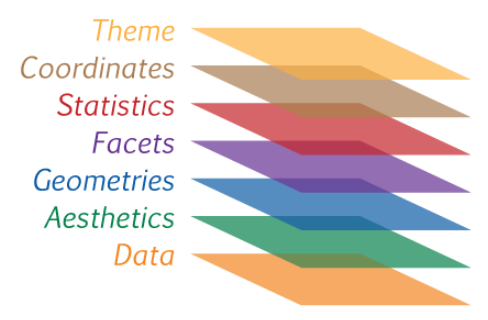
\includegraphics[width=\textwidth]{ggplot-layers.png}
Data, Aesthetics and Geometries are essential.
\end{frame}

\begin{frame}[fragile]\frametitle{ggplot2 - Grammar of Graphics}
Data
\begin{itemize}
\item The dataset being plotted
\begin{lstlisting}
ggplot(data=mydata100)
\end{lstlisting}
\item This does not show anything
\end{itemize}
\end{frame}

\begin{frame}[fragile]\frametitle{ggplot2 - Grammar of Graphics}
Aesthetics
\begin{itemize}
	\item How are variables \textbf{mapped} to visual properties of geometric objects?
	\item For example: x-axis, y-axis, color, fill, size, labels, alpha, shape, line width, line type
	\begin{lstlisting}
	ggplot(data=mydata100, aes(x=workshop))
	\end{lstlisting}
	\item This still does not show anything as it doesn’t know what geometry to apply
\end{itemize}
\end{frame}

\begin{frame}[fragile]\frametitle{ggplot2 - Grammar of Graphics}\footnotesize
Geoms: Geometric objects
\begin{itemize}
	\item The visual elements used for data, e.g. point, line, histogram, bar, boxplot	
	\begin{lstlisting}[basicstyle=\scriptsize]
	ggplot(data=mydata100, aes(x=workshop, fill=gender)) +
		geom_bar()
	ggplot(mydata100, aes(x=pretest, y=posttest)) +
 		geom_point()
 	ggplot(mydata3, aes(x=pretest, y=posttest,col=meanQ)) + 
 		geom_point()
	ggplot(mydata100, aes(x=pretest, y=posttest, col=workshop, size=q4)) + 
		geom_point()		
	ggplot(mydata3, aes(x=pretest, y=posttest, shape=workshop, col=meanQ, size=q4)) + 
		geom_point()		
	myboxplot <- ggplot(mydata100, aes(x=workshop, y=posttest)) +
		geom_boxplot()
	print(myboxplot)
	myboxplot +
		geom_point()
	ggplot(mydata100, aes(pretest,posttest, label = workshop)) + 
		geom_text()
	\end{lstlisting}
\item One great advantage of ggplot2: the plot is an object which can be manipulated!
\item Type \lstinline|geom_| and hit tab to see all possible values of OBJECT (which can be extended by other packages)
\end{itemize}
\end{frame}

\begin{frame}[fragile]\frametitle{ggplot2 - Grammar of Graphics}
Facets
\begin{itemize}
	\item Facets allow to put multiple charts / plots on one canvas by dividing into columns and rows
	\item Think of facets in terms of grouping your data
	\begin{lstlisting}
	p <- ggplot(mydata100, aes(x=posttest,fill=gender)) + 
		geom_histogram()
	p
	p +	facet_grid(. ~ gender)
	p +	facet_grid(gender ~ .)
	p + facet_grid(workshop ~ gender)
	\end{lstlisting}	
\end{itemize}
\end{frame}
\note{
\begin{itemize}
	\item different layers can even point to different data sets!
	\item so one data set could be raw data, another data set could be summary or confidence interval data
\end{itemize}
}




\begin{frame}[fragile]\frametitle{ggplot2 - Grammar of Graphics}
Statistics
\begin{itemize}
	\item Transformation or summary of your data before mapping to an aesthetic, e.g. binning, smoothing, descriptive, inferential
	\item Often the geom has default stats, which may work alright
	\item Sometimes providing a different stats does improve the clarity, e.g. calling
	\begin{itemize}
		\item \lstinline|stat_bin| instead of \lstinline|geom_bar| or \lstinline|geom_histogram|
		\item \lstinline|stat_smooth| instead of \lstinline|geom_smooth|
		\item \lstinline|stat_boxplot| instead of \lstinline|geom_boxplot|
	\end{itemize}  
	\item help of stat functions is often more informative
\end{itemize}
\begin{lstlisting}
p <- ggplot(mydata100, aes(x = pretest, y = posttest, col = gender)) + 
geom_point(alpha=0.4)
p +	geom_smooth()
p + geom_smooth(method="lm")
p + geom_smooth(method="lm",se=FALSE)
\end{lstlisting}
\end{frame}

\begin{frame}[fragile]\frametitle{ggplot2 - Grammar of Graphics}
Coordinates
\begin{itemize}
	\item Coordinate system controls how positions are mapped to the plot
	\begin{itemize}
		\item Cartesian coordinates
		\item Polar coordinates
		\item Spherical projection
	\end{itemize}
	\item Customization (and deception), e.g.:
	\begin{itemize}
		\item apply limits to x-axis or y-axis
		\item tune aspect-ratio
		\item zoom in
	\end{itemize}
\begin{lstlisting}
p <- ggplot(mydata100, aes(x = pretest, y = posttest, col = gender)) +
geom_point(alpha=0.4) +
geom_smooth()
p
p + scale_x_continuous(limits = c(65, 75)) #note the error message
p + coord_cartesian(xlim = c(65, 75)) # coord_cartesian(): the proper way to zoom in
\end{lstlisting}
\end{itemize}
\end{frame}

\begin{frame}[fragile]\frametitle{ggplot2 - Grammar of Graphics}
Theme
\begin{itemize}
	\item ggplot2 provides themes like \lstinline|theme_bw()|, \lstinline|theme_classic|, \lstinline|theme_dark|, \lstinline|theme_light|
	\begin{lstlisting}
p
p + theme_classic()
p + theme_dark()
p + theme_light()
p + theme_minimal()
p + theme_bw()
p + theme_grey()
p + theme_gray()
	\end{lstlisting}
	\item useful for corporate design, publication standards, personal choice
\end{itemize}
\end{frame}



\begin{frame}[fragile]\frametitle{ggplot2 - more examples}
More examples
\begin{lstlisting}[basicstyle=\footnotesize]
library(RColorBrewer)
myColors <- c("black", brewer.pal(4, "Dark2"))
ggplot(mydata100, aes(x = pretest, y = posttest, col = workshop)) +
	geom_point(alpha=0.8,shape="#") +
	geom_smooth(method = "lm", se = FALSE, fullrange=T) +
	geom_smooth(method = "lm",
					aes(group = 1, col = "All"), # Add col inside aes()
					se = FALSE, fullrange=T) +
	scale_color_manual("Participants", values = myColors)

load("recess.Rdata")
data("economics")
ggplot(economics, aes(x = date, y = unemploy/pop)) +
	geom_rect(data = recess,
				aes(xmin = begin, xmax = end, ymin = -Inf, ymax = +Inf),
				inherit.aes = FALSE, fill = "red", alpha = 0.2) +
	geom_line()
\end{lstlisting}
\end{frame}


\begin{frame}[fragile]\frametitle{ggplot2 - attributes}
More examples
\begin{lstlisting}
p <- ggplot(mydata100, aes(x=workshop, fill = gender))
p + geom_bar(position="fill")
p + geom_bar(position="stack")
p + geom_bar(position="dodge")
p +  geom_bar(position = position_dodge(0.2), alpha = 0.6)
p + geom_bar(position="fill") +
scale_fill_grey()

library(RColorBrewer)
display.brewer.all(n=5) # how many column patterns
p + geom_bar(position = "stack") + 
	scale_fill_brewer(palette = "Set2")
\end{lstlisting}
\end{frame}

\begin{frame}[standout]
Exercise 16 and 17
\end{frame}


\section{Cleaning Data}
\begin{frame}[fragile]\frametitle{Missing Values}\footnotesize
\begin{itemize}
	\item Missing values are neither negative nor positive infinity like in STATA
	\item \lstinline|Inf| is infinity, also a kind of missing value, and you CAN do size comparison to it
	\item Finding missing values:
	\begin{itemize}\footnotesize
		\item Not \lstinline|x == NA| but \lstinline|is.na(x)|
		\item Counting missing values:
		\begin{lstlisting}[basicstyle=\footnotesize]
		x <- c(NA,2,NA,2,1)
		length(x)      #number of all variables
		sum(is.na(x))  #number of missing values
		sum(!is.na(x)) #number of valid values
		\end{lstlisting}
	\end{itemize}
	\item Hint: have a look at \lstinline|valid.n()| from the \lstinline|prettyR| package
		\begin{lstlisting}[basicstyle=\footnotesize]
		library(prettyR)
		valid.n(x)
		\end{lstlisting}
		 or write your own function:
		\begin{lstlisting}[basicstyle=\footnotesize]
		n.missing <- function(x){
			sum(is.na(x))
		}
		n.missing(x)		
		\end{lstlisting}
	
\end{itemize}
\end{frame}


\begin{frame}[fragile]\frametitle{Missing Values}
Setting values to missing
\begin{itemize}
\item R reads numeric blanks as missing
\item Remember: when creating factors, non-specified levels will become missing values
\item When reading text files you can specify NA by option\newline
\lstinline|na.string = c(".","99","999")|
\item Better: use conditional transformations:\\ \lstinline|age[age == 999] <- NA|
\end{itemize}
\end{frame}
\note{na.strings affects all columns of your data set, and the missing values might be different for different values, so better use conditional transformations}

\begin{frame}\frametitle{Action on Missing Values}
\begin{itemize}
\item Summary functions return \lstinline|NA| unless \lstinline|na.rm=TRUE|
\item Modeling functions (that accept formula) automatically exclude \lstinline|NA|s
\item Replacing/Imputing missing values
\begin{itemize}
\item \lstinline|VIM| (Visualization and Imputation of Missing Values): useful to find patterns in missing values and visualize them in color maps (\lstinline|colormapMiss()|), bar charts (\lstinline|barMiss()|) and histograms (\lstinline|histMiss()|)	
\item \lstinline|mice| (Multivariate Imputation by Chained Equations): \lstinline|md.pattern()| function also searches for patterns of missing values
\end{itemize}
\end{itemize}
\end{frame}

\begin{frame}[standout]
Exercise 18
\end{frame}

\section{Linear regressions}


\begin{frame}
\frametitle{Multiple linear regression}
\begin{itemize}
	\item The general syntax of regression models is rather idiosyncratic:
\end{itemize}
\begin{center}
	\texttt{a <- lm(formula)}
\end{center}
\begin{itemize}
	\item Basic \textquotedblleft formula\textquotedblright\ syntax
\end{itemize}
\begin{center}
	\texttt{y \symbol{126} x1 + x2 + \ldots\ + xK}
\end{center}
\begin{itemize}
	\item Endogenous variable is on the left of \texttt{\symbol{126}}; exogenous
	variables are on the right of \texttt{\symbol{126}}, separated by \texttt{+}
	\item In R modeling functions: accept formulas, create model objects, generic functions show more, extractor functions show more
	
\end{itemize}
\end{frame}


\begin{frame}[fragile]
\frametitle{Multiple linear regression}
Example
\begin{lstlisting}
library(foreign)
x <- read.dta("wave2009.dta")
attach(x)
regr1 <- lm(satisfaction ~ age + netincome + children)
regr1
plot(regr1)
summary(regr1)
names(regr1)
print(unclass(regr1))
\end{lstlisting}
\end{frame}


\begin{frame}
\frametitle{Multiple linear regression}
\begin{itemize}
\item The \texttt{lm}-object is a list containing:
\begin{enumerate}
\item The estimated coefficients $\hat{\beta}$
\item The residuals $\hat{u}_{t}$
\item The fitted values $\hat{y}_{t}$
\item Some other things
\end{enumerate}
\item If \texttt{a} is an \texttt{lm}-object one can access its elements
using\newline
\texttt{coefficients(a)}, \texttt{residuals(a)}, \texttt{fitted.values(a)}
\item Alternatively, one can use the \texttt{\$}-operator: \texttt{%
a\$coefficients}, \texttt{a\$residuals}, \texttt{a\$fitted.values}
\end{itemize}
\end{frame}


\begin{frame}
\frametitle{Multiple linear regression}
Extensions (I):
\begin{itemize}
\item An intercept is added automatically but can be removed: \texttt{lm(y\symbol{126}x1+x2-1)}
\item If the variables are organized in an unattached dataframe \texttt{x}, 
\newline
one can use the syntax: \texttt{lm(formula,data=x)}
\item The formula may contain mathematical functions, e.g. \texttt{lm(log(y)%
\symbol{126}log(x1))}
\item \textbf{Attention}: Squares, sums and differences are not allowed!
\item Use the function \texttt{I()} for squares, sums and differences
\end{itemize}
\end{frame}


\begin{frame}[fragile]
\frametitle{Multiple linear regression}
Extensions (II):
\begin{itemize}
\item Syntax for interaction terms
\end{itemize}
\begin{center}
\texttt{a <- lm(y \symbol{126} x1 + x2 + x1:x2)}
\end{center}
\begin{itemize}
\item Abbreviations:
\begin{itemize}
\item \lstinline|a <- lm(y ~ x1*x2)|
\item \lstinline|a <- lm(y ~ (x1+x2)^2)| for all interactions up to 2
\end{itemize}
\item Weights can be added using the option \texttt{weights}
\item One can select a subset of observations using the option \texttt{subset}
\end{itemize}
\end{frame}


\begin{frame}[fragile]
\frametitle{Multiple linear regression}
Extensions (III):
\begin{itemize}
\item The \texttt{lm}-object can be used to add a regression line to a plot:
\begin{lstlisting}
regr <- lm(y~x)
plot(x,y)
abline(regr)
\end{lstlisting}
\item The \texttt{lm}-object can be used for forecasting:
\begin{lstlisting}
regr <- lm(y~x1+x2)
xn <- data.frame(x1=c(...),x2=c(...))
predict(regr,newdata=xn,se.fit=TRUE)
\end{lstlisting}
\end{itemize}
\end{frame}


\begin{frame}[fragile]
\frametitle{Multiple linear regression}
Extensions (IV):
\begin{itemize}
\item Heteroskedasticity consistent standard errors are not reported by default
\item The package \texttt{lmtest} supplies functions for robust standard errors
\item The syntax for robust standard errors is
\end{itemize}
\begin{lstlisting}
coeftest(regr,vcov=vcovHC)
\end{lstlisting}
\end{frame}

\begin{frame}[fragile]\frametitle{Polynomial regression}
Polynomial regression
\begin{lstlisting}
y ~ x + I(x^2) + I(x^3)
y ~ poly(x,3)
\end{lstlisting}
\end{frame}
\note{I means isolates this call}

\begin{frame}[fragile]
\frametitle{Multiple linear regression}
Putting it all together:
\begin{lstlisting}
regr2 <- lm(satisfaction~age+netincome,data=x)
regr3 <- lm(satisfaction~age+I(age^2))
regr4 <- lm(satisfaction~log(netincome))
regr5 <- lm(satisfaction~gender*marital)
z <- gender=="Female"
regr6 <- lm(satisfaction~log(netincome),subset=z)
library("lmtest")
coeftest(regr6,vcovHC)
\end{lstlisting}
\end{frame}



\begin{frame}[standout]
Exercise 19 and 20
\end{frame}

\section{Programming} 
\begin{frame}
\frametitle{User-defined functions}
\begin{itemize}
\item One can define new functions in R
\item Functions are objects of class \texttt{function}
\item Each function has a name, one or more inputs (arguments) \newline
and one output (return)
\item Inputs can be any objects (usually vectors)
\item The function can return only one object (which can be a list)
\item Variables defined within a function are only local
\end{itemize}
\end{frame}
\note{similar to macros}


\begin{frame}
\frametitle{User-defined functions}
Syntax\medskip

\texttt{fn <- function(x,y)\{}

\quad \texttt{block of commands to compute output out}

\quad \texttt{return(out)}

\quad \texttt{\}\bigskip}
\begin{block}{Example}
\texttt{utility <- function(cons,gam)\{}

\quad \texttt{U <- (cons\symbol{94}(1-gam)-1)/(1-gam)}

\quad \texttt{return(U)}

\quad \texttt{\}}
\end{block}
\end{frame}

\begin{frame}[fragile]
\frametitle{User-defined functions}
Example
\begin{lstlisting}
mystats <- function(x) {
	mymean <- mean(x, na.rm=TRUE)
	mysd   <-   sd(x, na.rm=TRUE)
	c(mean=mymean, sd=mysd) #only last thing is remembered
}
mystats(posttest)
mymean #not found
\end{lstlisting}
\begin{itemize}
\item functions return only a single object, the last one created, but can contain many results
\item applying functions by group
\begin{lstlisting}
by(posttest, workshop, mean)
by(posttest, workshop, mystats)
\end{lstlisting}
\end{itemize}
\end{frame}


\begin{frame}[standout]
Exercise 21
\end{frame}




\begin{frame}[fragile]
\frametitle{Loops}
\begin{itemize}
\item If the same commands should be executed for different values of some
variable, loops are useful
\item There are three kinds of loops: \texttt{for}, \texttt{while}, \texttt{repeat}
\item By far the most important loop is the \texttt{for}-loop
\item General syntax:
\end{itemize}
\begin{verbatim}
    for([var] in vector) {
        [commands]
    }
\end{verbatim}
\begin{itemize}
\item The commands are executed for each value of \texttt{vector}
\end{itemize}
\end{frame}


\begin{frame}[fragile]
\frametitle{Loops}
Example
\begin{lstlisting}
z <- rep(NA,10)
for(i in 1:10) {
  z[i] <- i^2
}
print(z)
\end{lstlisting}
\end{frame}


\begin{frame}
\frametitle{Loops}
\begin{itemize}
\item Syntax of the \texttt{while}-loop:
\end{itemize}
\begin{center}
\texttt{while([condition]) \{[commands]\}}
\end{center}
\begin{itemize}
\item Syntax of the \texttt{repeat}-loop:
\end{itemize}
\begin{center}
\texttt{repeat \{[commands]\}}
\end{center}
\begin{itemize}
\item The \texttt{repeat}-loop does never stop but can be left using the
command \texttt{break}
\end{itemize}
\end{frame}


\begin{frame}[fragile]
\frametitle{Conditions}
Syntax of the \texttt{if}-command
\begin{verbatim}
    if([condition]) {
       [commands]
    }
\end{verbatim}
\begin{itemize}
\item The condition must not be a vector
(else only its first element is used)
\item If there is just a single command, the brackets can be omitted
\item The opening curly bracket must appear in the same line as the \texttt{%
if}-command
\item It is possible to add \texttt{else \{[commands]\}}
\end{itemize}
\end{frame}


\begin{frame}
\frametitle{Random numbers}
\begin{itemize}
\item A large number of standard distributions is implemented in R
\item There is a common syntax for cdfs, density functions, quantile
functions, and random number generation:
\begin{description}
\item[\texttt{pNAME(x,pars)}] cumulative distribution function at $x$
\item[\texttt{dNAME(x,pars)}] density (or probability) function at $x$
\item[\texttt{qNAME(p,pars)}] quantile function at $p$
\item[\texttt{rNAME(n,pars)}] generate $n$ random draws
\end{description}
\item Here \texttt{NAME} is the abbreviated name of the distribution and 
\texttt{pars} are its parameters
\end{itemize}
\end{frame}


\begin{frame}
\frametitle{Random numbers}
\framesubtitle{Standard distributions}
Some continuous distribution names:
\begin{description}
\item[\texttt{norm}] normal
\item[\texttt{unif}] uniform
\item[\texttt{lnorm}] log-normal
\item[\texttt{exp}] exponential
\item[\texttt{t}] $t$-distribution
\item[\texttt{chisq}] $\chi ^{2}$-distribution
\item[\texttt{F}] $F$-distribution
\end{description}
\end{frame}


\begin{frame}
\frametitle{Random numbers}
\framesubtitle{Standard distributions}
Some discrete distribution names:
\begin{description}
\item[\texttt{binom}] binomial
\item[\texttt{pois}] Poisson
\item[\texttt{geom}] geometric
\item[\texttt{hyper}] hyper-geometric
\item[\texttt{nbinom}] negative binomial
\item[\texttt{multinom}] multinomial
\end{description}
\end{frame}


\begin{frame}
\frametitle{Random numbers}
\framesubtitle{Standard distributions}
\begin{itemize}
\item Define a vector $x$ on an appropriate grid $[a,b]$
\item Plots of cdf and density functions:
\end{itemize}
\begin{center}
\texttt{plot(x,pNAME(x,pars))}

\texttt{plot(x,dNAME(x,pars))}
\end{center}
\begin{itemize}
\item Define a grid vector $p$ on $[0,1]$; plot of quantile function:
\end{itemize}
\begin{center}
\texttt{plot(x,qNAME(p,pars))}
\end{center}
\end{frame}


\begin{frame}[fragile]
\frametitle{Simulations}
Example: Simulate the distribution of the moment estimator of the exponential distribution
\begin{lstlisting}
R <- 10000
Z <- rep(NA,R)
for(r in 1:R) {
  x <- rexp(n=10,rate=0.5)
  Z[r] <- 1/mean(x)
}
truehist(Z)
abline(v=2,col="red")
\end{lstlisting}
\end{frame}

\begin{frame}[standout]
Exercises 22, 23, and 24
\end{frame}





\section{High Quality Output}

\begin{frame}[fragile]
\frametitle{High Quality Output}
\begin{itemize}
\item Paste into word processor
\item Use packages, e.g. xtable and texreg
\item rtf or R2DOCX to write complex Word docs, but hard to set up
\item Reproducable research: knitr and rnotebook
\end{itemize}
\end{frame}

\begin{frame}[fragile]\frametitle{High Quality Output}
Example
\begin{lstlisting}
myM1 <- lm(q4 ~ q1 + q2 + q3, data=mydata100)
myM2 <- lm(q4 ~ q1, data=mydata100)

library("xtable")
print(xtable(myM1),type="html",file="myM1-xtable.doc")

library("texreg")
htmlreg(myM1, single.row=TRUE,file="myM1-htmlreg.doc")
htmlreg(list(myM1,myM2), file="myM1-myM2-htmlreg.doc")

texreg(list(myM1, myM2))
\end{lstlisting}
\end{frame}
\end{document}
